\subsection{Definitions}
\begin{itemize}
	\item \textbf{Pervasive Computing}
	\begin{itemize}
		\item Pervasive Computing $\approx$ Ubiquitous Computing
		\item pervasive = \textit{alles durchdringend}
		\item IBM-Definition: \glqq Convenient access, through a new class of appliances, to relevant information with the ability to easily take action on it when and where you need\grqq
		\item Beispiel: Smartphones $\rightarrow$ relativ neue Technologie, daher viel höhrere Dynamik in der Entwicklung als beim Desktop. 
		\item Implizite Interaktionen: Gerät reagiert implizit auf User-Aktivität (insbesondere bei Smart Homes), jüngere lernen das besser (je älter man wird, desto mehr muss man anhand von Bezügen zu bereits Gelerntem/Metaphern lernen)
	\end{itemize}
	\item \textbf{Human Adopted Production}
	\begin{itemize}
		\item Comber and Maltby (1997) found that both overly simple and overly complex computing interfaces were low in usability 
		\item Wie kann man den User \glqq bei Laune halten\grqq ?\\
	 	$\rightarrow$ Die aktuell erfahrene Komplexität muss im Mittelmaß sein\\
	 	$\rightarrow$ Lernsysteme greifen per GSR Stress Level des Users ab und tunen dementsprechend das Lernsystem\\
	 	$\rightarrow$ kognitive Paramater sind sehr individuell
		\begin{figure}[h!]
			\centering
			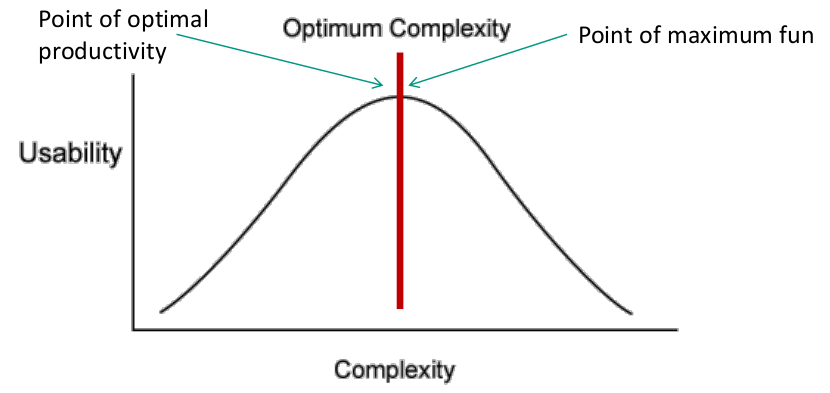
\includegraphics[width=.4\textwidth]{img/ch01_HAP.png}
			\caption{Human Adopted Production}
			\label{HAP}
		\end{figure} 
	\end{itemize}
	\item \textbf{Human-Computer-Interaction}
	\begin{itemize}
		\item Important part of Pervasive Computing, e.g. Mobile Phone interfaces
		\item Pervasive Computing Technology produces now most/all innovative human machine interfaces, e.g. augmented reality glasses
		\item everything you see, touch, feel, do... to exchange information with a technical system
		\item Wikipedia: “Human-Computer interaction (HCI) is the study of interaction between people (users) and computers. It is an interdisciplinary subject, relating computer science with many other fields of study and research. Interaction between users and computers occurs at the user interface (or simply interface), which includes both hardware (i.e. peripherals and other hardware) and software (for example determining which, and how information is presented to the user on a screen).”
		\item SIG CHI: “Human-computer interaction is a discipline concerned with the design, evaluation and implementation of interactive computing systems for human use and with the study of major phenomena surrounding them.”
	\end{itemize}
\end{itemize}
\subsection{Applications}
\begin{itemize}
	\item Reprogramming Senses: Proximity Helmet (mit Arduino) $\rightarrow$ wird nach einer Weile zum Gefühl, so kann man neue Sinne erschaffen
	\item Augmented Reality, Mobile Computing User Interface Software Design
	\item Wearable Thermography: detektiert Überbelastung bei Sport...
	\item Ubiquitous Sensing: Lobster House, Büro welches sich nach Sonne dreht, jeder Quadratmeter individuell klimatisierbar
\end{itemize} 

\subsection{Interactive Systems Design}
An interactive systems designer needs: 
\begin{itemize}
\item Knowledge about people: Sociology, anthropology, psychology, culture
\item Knowledge about technologies: Software, systems, electronics, communications, materials, databases, etc.
\item Knowledge about activities and contexts: Communities of practice, information systems, organizations, knowledge management
\item Knowledge about design: Fashion, interior, information design, architecture, product design
\end{itemize}
\textbf{Design}: The creative process of specifying something new and the representations that are produced along the way (e.g. site map, blueprints, sketches, etc.). It typically involves much iteration -- both problem and solution evolve during design. Design is a spectrum of activities:
\begin{itemize}
\item Engineering design -- using scientific principles: Architect designs buildings, urban planner designs roads, etc.
\item Artistic design: Creative design where imagination is key
\item Design as craft: Design is a `conversation with materials',  e.g. pottery designer works with clay, clothes designer works with fabrics, interior designer works with furniture, paints, lighting, etc.
\end{itemize}

\subsection{PACT}
PACT is a framework for designing interactions. People undertake activities, in contexts using technologies.\\
\begin{figure}[h!]
			\centering
			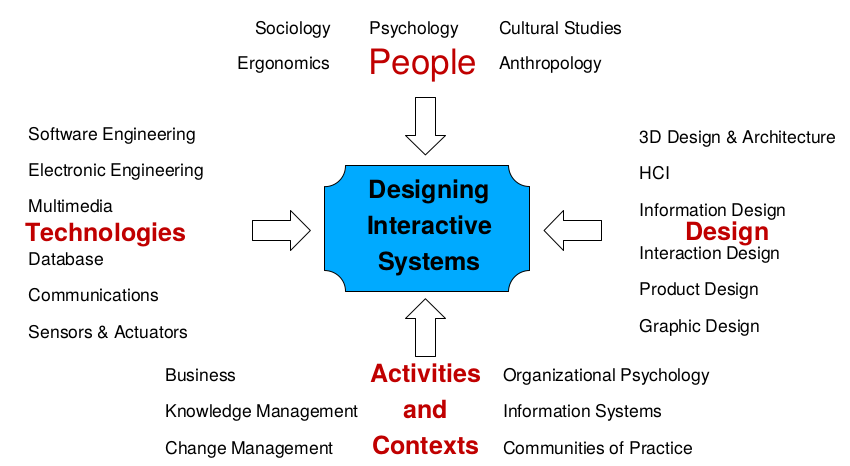
\includegraphics[width=.6\textwidth]{img/ch01_pact.png}
			\caption{PACT method}
			\label{pact}
\end{figure} 
\textbf{People}:
\begin{itemize}
\item Physical differences: Height, weight, different capabilities in sight, hearing, touch,...
\item Psychological differences: Different ways of working; different memory abilities (short term and long term) and spatial ability; different amounts of attention at different times; differences in perception and attention and -- crucially -- different `mental models' 
\begin{itemize}
\item Mental Model: A mental representation of a real-world object or process, a set of associations with it. Describes the ways in which we think about things - about how we conceptualize things.\\
$\rightarrow$ A key aspect of the design of technologies is to provide people with a clear model, so that they will develop a clear mental model but of course that depends on what they know already, their background, experiences, etc. etc.
\end{itemize}
\item Usage differences: Experts versus novices, discretionary users of technologies, differences in designing for a heterogeneous group or a homogeneous group
\end{itemize}
\textbf{Activities}:
\begin{itemize}
\item Temporal aspects: How regular or infrequent are the activities? Continuous set of actions, or can be interrupted? Response time\footnote{100ms for hand-eye coordination activity, 1 second for cause-effect activity, over 5 seconds and people quickly get frustrated.} from the system?
\item Co-operation and Complexity: Working with others or not?
\item Safety critical: What problems happen if something goes wrong?
\item Content: What information and media are we dealing with?
\end{itemize}
\textbf{Contexts}:
\begin{itemize}
\item Physical environment is one sort of context: e.g. ATM or ticket machine versus computer at home
\item Social context is important: Help from others, acceptability of certain designs
\item Organizational context: Power structure, changes in life style, etc.
\end{itemize}
\textbf{Technologies}: 
\begin{itemize}
\item Input: Some methods are needed to enter commands (tell the system what we want it to do). We also need to be able to navigate through the commands and the content of the system. We need to enter data or other content into the system. The medium needs to be suited for different contexts/activities.
\item Output: The system has to tell us what is happening, i.e. provide feedback. It has to be able to display the content to us. 
\item Communication: Between person and technology and between devices $\rightarrow$ Bandwidth, speed
\item Content: Functional systems versus systems more focused on content
\end{itemize}
When doing a PACT analysis, \textbf{scenarios} are good for \textbf{evaluation and envisionment}. Scenarios are stories about people undertaking activities using technologies in contexts. You start to develop conceptual scenarios that cover the main activities that the technology has to support. Then you develop concrete versions of these for specific designs of the technology. E.g. a conceptual scenario might say `Pete logs onto the computer' and a concrete version might be `Pete clicks on the \textit{log on} icon'.\\
A \textbf{Persona} is a profile of an archetypal person in the domain. Personas are synthesized from knowledge of real people in the domain. They need to have goals -- describe what they are trying to achieve. Like scenarios, conceptual personas are abstract types -- students, lecturers, etc. For design it is best to develop a few concrete personas who have hard characteristics such as age, interests, a name, etc. Try to bring the character alive -- perhaps including pictures.


